\section{MVC}
Quando trattiamo il pattern MVC, quello a cui ci riferiamo è una soluzione architetturale che si compone di tre elementi principali:
\begin{itemize}
    \item \textbf{Model}: è implementato dalle classi che realizzano la logica applicativa dell’applicazione.  \\
      Viene indicato dalle applicazioni web come backend. Contiene l’API e le classi che implementano l’API, quindi le funzionalità che l’applicazione deve offrire e contiene anche la rappresentazione dei dati.
      Incapsula lo stato dell’applicazione (dati memorizzati, entità e il loro stato) e risponde a query sullo stato.
      Espone le sue funzionalità dell’applicazione e notifica le views di eventuali cambiamenti.
    \item \textbf{View}: ciò che viene mostrato all’utente.\\ 
      Presenta il contenuto informativo e lo stato del model. Esegue il rendering dei modelli e ne riceve gli update. Manda le gesture degli user al controller e permette al controller di selezionare la view.
    \item \textbf{Controller}: serve per controllare l’interazione tra model e view.
      Definisce il comportamento dell’applicazione.
      Mappa le azioni utenti in update del modello.
      Seleziona la vista con cui rispondere.
      Esiste un controller per ogni funzionalità.
\end{itemize}
La \textit{view} raccoglie gli input dell’utente (user gesture) e li inoltra al controller che le mappa in operazioni sul modello.
Il model viene modificato e il controller sceglie la successiva view da mostrare che si occuperà di fare il rendering dello stato dell’applicazione.
Per poter fare il rendering dello stato del model, la view deve accedere al model per ottenere le informazioni di stato.
Ci possono essere dei cambiamenti di stato spontanei nel model che devono essere notificati alla view che deve adattarsi al nuovo stato.
\begin{figure}[H]
    \centering
    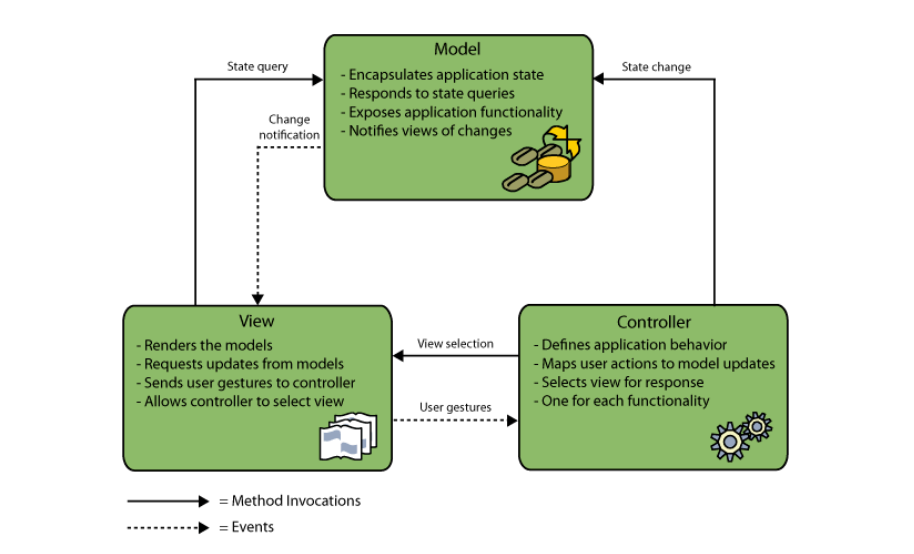
\includegraphics[scale=0.6]{Imm/mvc-archi.PNG}
\end{figure}

Nella pratica, nelle pagine HTML statiche, la view è il browser, il controller è il web server e il model sono i file html e i file di stile. Quello che succede, è che le richieste vengono inoltrare attraverso un URI, questo è uno standard attraverso il quale possiamo inviare query nella forma $urlPagina/?name=Alice\&altro=Bob$. Quello che ci viene ritornato sono dati risedenti sul web server(magari presenti in un campo hidden). \\

Nelle pagine dinamiche invece, il model è la logica di business (o logica applicativa) (ad esempio un’implementazione Java), la view è il rendering dei dati dell’applicazione (ad esempio pagine JSP) e il controller è la presentazione logica (ad esempio le servlet).

\subsection{HTML Forms}
Trasmettono le informazioni dai Web Browsers alle Web applications (URI + dati), solitamente sotto forma di elementi FORM.\\ Gli attributi che vengono considerati sono:
\begin{itemize}
   \item ACTION, che processa i dati, 
   \item METHOD che se è impostato a GET, invia i dati attraverso il l’URI, mentre se è a POST, manda i dati nel body.
   
\end{itemize}
\subsection{Servlet}
Componente Web Java-based progettato per generare contenuti dinamici. NEl caso illustrato si nota facilmente come attraverso il Browser, che ricordiamo sia la nostra view, inoltriamo delle richieste HTTP alla Servlet (Che non è il nostro WebServer, ma è una componente del server Applicativo. Pensiamo ad esempio a una JSP che si appoggia su tomcat per gestire le richieste.)
\begin{figure}[H]
    \centering
    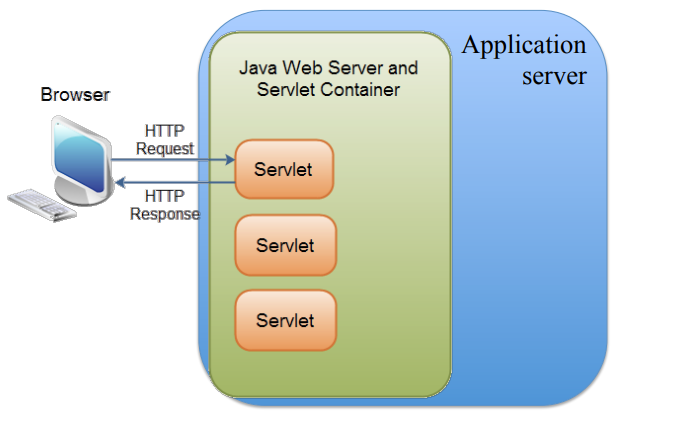
\includegraphics[scale=0.6]{Imm/jsp-servlet.PNG}
\end{figure}

\subsubsection{Ciclo di vita di una servlet} 
gestito dal container

\begin{figure}[H]
    \centering
    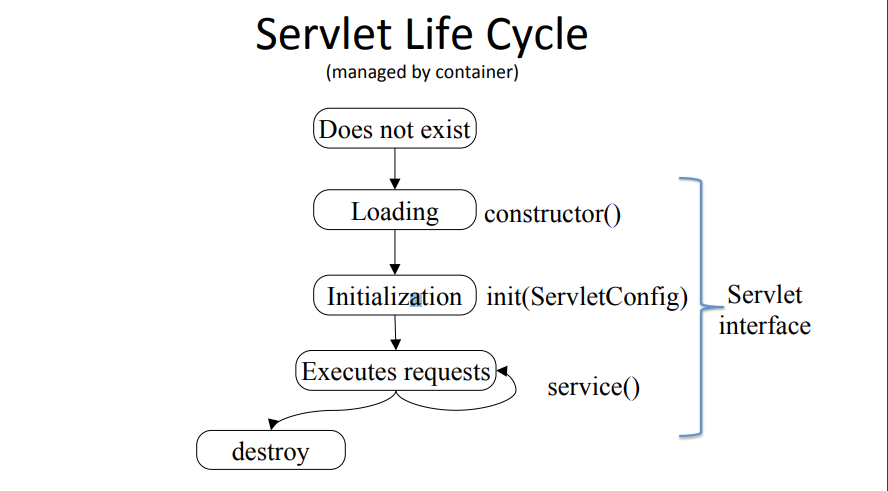
\includegraphics[scale=0.6]{Imm/servlet-life.PNG}
\end{figure}

\begin{lstlisting}
    //HttpServlet class
    abstract class HttpServlet implements Servlet
        
    //metodi aggiuntivi
    doPost(HttpServletRequest, HttpServletResponse)
    doGet(HttpServletRequest, HttpServletResponse)
\end{lstlisting}


Per gestire le richieste, si implementa \textit{HttpServletRequest} che dà un significato ai parametri della get request (dati utente inseriti in una form). Per reperire informazioni: \textit{Object user = request.getParameter("user")}\\
Il tempo di vita di un oggetto richiesto è limitato dal metodo \textit{service()} della servlet.

\subsection{Cookies}
Piccola stringa che può essere memorizzata in un client. Possono essere usati per identificare un user con una sessione web di lunga durata, per memorizzare alcuni dati interessanti sul client (nickname, id, numero di carta), per personalizzare il sito sulla base del profilo utente.\\
Il browser restituisce un set di cookies al sito e la Web applications utilizza le loro informazioni nella sua logica.

\begin{lstlisting}
    //To create cookies
    Cookie c = new Cookie('name', 'value');
    resp.addCookie(c;)
    //To get cookies
    Cookie cArray[] = req.getCookies();
\end{lstlisting}


\subsection{Session}
Una sessione è una serie di richieste associate una all’altra. Mantenere una sessione è difficile a causa della natura del protocollo HTTP.\\
Esistono diversi meccanismi per tracciare sessioni differenti: cookies, URL rewriting e hidden form fields. È il server che si occupa di gestire le sessioni.

\begin{lstlisting}
    //Getting session
    Session session = req.getSession(true);
    //Storing session infomartion in session 
    session.getAttribute(name, valueObject);
    //Retrieving information from session
    session.getAttribute(name);
\end{lstlisting}

\subsection{Sharing Data}
Ci sono diversi posti dove le servlet possono memorizzare e recuperare i dati.

\begin{table}[H]
    \centering
    \begin{tabular}{|l|l|}
        \hline
        \textbf{Place} & \textbf{Scope}                         \\ \hline
        Request        & Esecuzione del metodo service          \\ \hline
        Session        & Richieste multiple da un stesso utente \\ \hline
        ServletContext & Application-wide                       \\ \hline
    \end{tabular}
\end{table}
\textbf{Application-wide} significa che i dati devono poter essere accessibili attraveso tutta l'applicazione in modo condiviso. Stessa situazione si ha quando si usa \textit{Application Context} all'interno delle applicazioni Android.

\subsection{Threading}
Una servlet per container condivide tra multipli user e richieste, gestisce il multiThreading e presta attenzione quando accede ai dati nella sessione e nel contesto della sessione.

\subsection{JSP (Java Server Pages)}
Servono per incorporare elementi dinamici nella pagine web statiche.
Le pagine JSP sono compilate nelle servlet Java prima di essere eseguite.
(Richiesta di una pagina, generazione di una servlet da una pagina JSP, memorizzazione di una servlet per un utilizzo successivo, esecuzione di una servlet)

\begin{lstlisting}
<%=%> //JSP expression: usata per visualizzare una variabile Java
<% %> //JSP Scriplet: usata per il codice Java normale 
\end{lstlisting}

\subsubsection{Tag Libraries}
JSP supporta l’uso di librerie di tag standard e personalizzabili.
\begin{lstlisting}
<%@ taglib uri = "URIToTagLibrary" prefix="tagPrefix" %>
\end{lstlisting}

\subsection{Design Patterns}
Ci sono diversi Design Pattern, ogni pattern risolve, in lineea di massima, un determinato tipo di problema che ci si presenta.
\begin{itemize}
    \item \textbf{Controller Design}
    \begin{itemize}
        \item \textbf{Page Controller} si implementa un controller per ogni pagina.\\
         Responsabilità principali: controllare i parametri di richiesta e invoca la logica di business, selezionare la prossima vista da mostrare e preparare i dati per la presentazione.\\

        Control flow: il controllo si sposta dalla Web Server al PageController, che estrae i parametri dalla richiesta, utilizza dei business object, decide la view successiva, prepara i dati da mostrare nella view successiva e infine cede il controllo e i dati alla View.\\
        Possibili implementazioni: server page (ASP, JSP, PHP), con poca logica di controllo, o script (CGI script, servlet), con una logica di controllo significativa.\\
        È scalabile.
        \item \textbf{Front Controller} a differenza del Page controller, il Font Controller è un componente singolo che riceve le richieste da tutte le componenti della view.
        Definisce un singolo componente che gestisca tutte le richieste, eseguendo prima le operazioni comuni a tutte le richieste e poi quelle specifiche.\\
        Si divide in: 
        \begin{enumerate}
            \item \textit{Handler}: riceve le richieste dal server, esegue le operazioni generali/comuni, decide le operazioni che devono essere eseguite e delega l’esecuzione al Concrete Command.
            \item \textit{Concrete Command}: estrae i parametri dalla richiesta, invoca i metodi implementati nella logica di business, determina la view successiva e cede il controllo alla View.
        \end{enumerate}
        Il Front Controller è più complesso del Page Controller, evita che ci sia codice duplicato tra i controller, facilita la configurazione del server (solo una servlet), ha la possibilità di gestire dinamicamente nuovi comandi e è facile estendere il controller (perché ce n’è solo uno).\\
        In alcuni casi, i comandi possono essere implementati come metodi anziché come classi.\\
        È scalabile.
        \item \textbf{Intercepting Filter} 
        Utile per gestire le richieste e le risposte prima che vengano soddisfatte.
        Spesso usato con Front Controller, per aggiungere alle richieste e alle risposte funzioni aggiuntive come il logging, l’autenticazione, la conversione dei dati e l’internazionalizzazione.
        \begin{figure}[H]
            \centering
            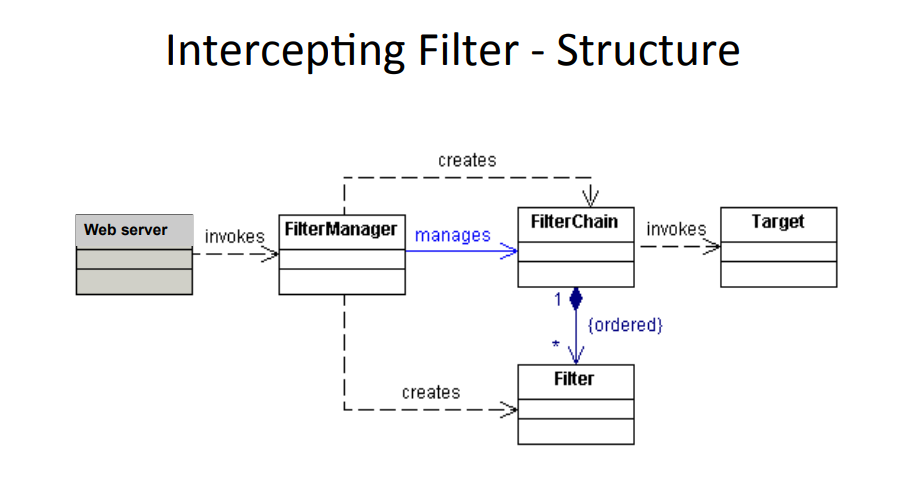
\includegraphics[scale=0.6]{Imm/if-struttura.PNG}
        \end{figure}
        Il Web Server solitamente fornisce il FilterManager e il FilterChain; quindi c’è solo bisogno di implementare e dichiarare i Filtri.
        \begin{figure}[H]
            \centering
            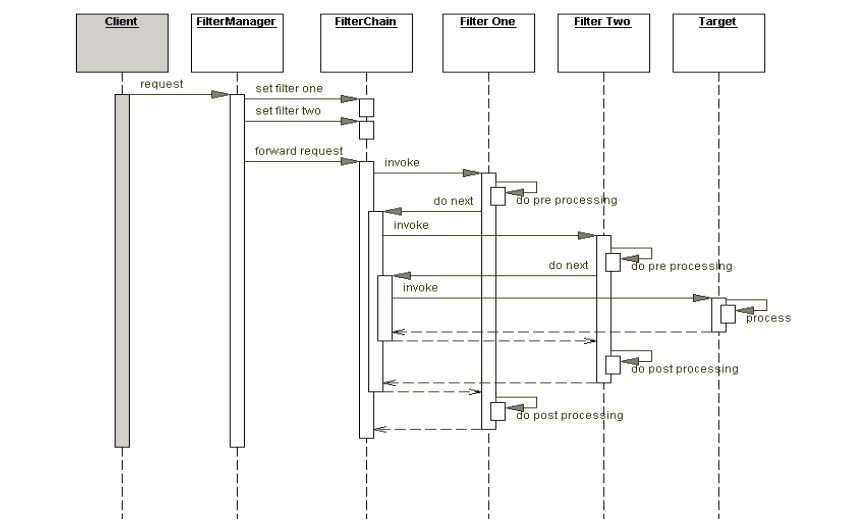
\includegraphics[scale=0.6]{Imm/if-behave.PNG}
            \caption{Qui possiamo notare in un diagramma a sequenza le varie interazioni che si hanno a Partire dal Client fino al raggiungimento del Target}
        \end{figure}
        \item \textbf{Application Controller}: Quando cresce la complessità del flow, il management del flow potrebbe essere concentrato in una classe.
         \begin{figure}[H]
            \centering
            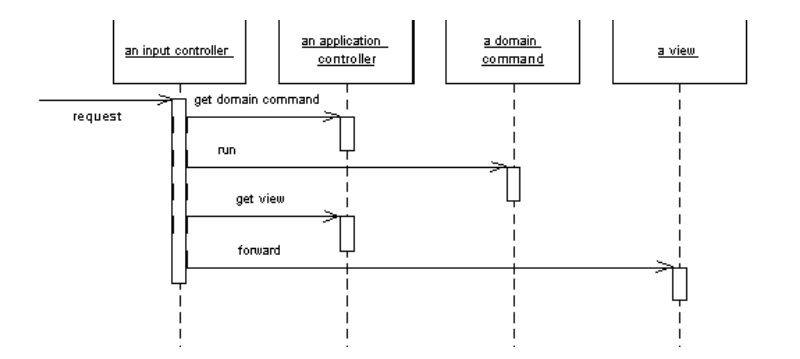
\includegraphics[scale=0.6]{Imm/ac-diagram.PNG}
            \caption{Questa tipologia di approccio viene tipicamente utilizzata dal Page Controller o dal Front Controller}
        \end{figure}
    \end{itemize}
    \item \textit{View Design}, una seconda categoria di pattern, che riguarda più la costruzione delle pagine invece che concentrarsi sul controllo di dati.
    \begin{itemize}
        \item \textbf{ Template View}: La parte di rendering viene ottenuta definendo parte di contenuto statico e parte di contenuto dinamico il cui effettivo valore dipende dal modello e dal suo stato. \\
        Utilizza le classi Helper create dal Controller, per facilitare la costruzione della pagina: la pagina non fa diretto accesso al modello ma fanno riferimento all’Helper che a sua volta fa riferimento al Model. L’Helper prepara dei dati ad hoc per la parte di presentazione.\\
        Il Block-helper genera codice HTML dalle pagine di template che includono chiamate al modello. Genera i dati di dominio, separa la View dall’implementazione logica ed è creato da un controller e acceduto da una View.
        \item \textbf{Transformation View}  Non si ha una pagina template con parti costanti e parti dinamiche ma la pagina viene creata interamente in modo dinamico a partire dai dati che devono essere presentati. Il componente responsabile per la costruzione di questa pagina è il Transformer.\\
        Trasforma le entità di dominio in HTML. Una tipica implementazione del modello è quella in cui ogni classe di dominio implementa la funzione toXML(). Una tipica implementazione del Transformer usa XSLT (eXtensible Style), un linguaggio per le trasformazioni.\\
        Transformation View si focalizza sull’entità che dev’essere trasformata piuttosto che sulla pagina di output (Template View).\\
        È difficile da includere l’implementazione logica nella View; è però facile da testate (controllando lo stream che si genera dopo la trasformazione XSLT) ed è facile da applicare a dati XML.\\
        WYSIWYG è più intuitivo e facile da gestire.
        \item \textbf{Two-Steps View} Genera la pagina HTML in due steps: genera una pagina logica e renderizza la pagina.\\
        Appare facile da modificare perché il rendering non interferisce con la struttura dell’informazione che dev’essere visualizzata sulla pagina.
        L’implementazione consiste nella sequenza di due trasformazioni XSLT: costruire la pagina logica e renderizzare la pagina.
        La Templete View ha dei tag personalizzabili.
        Quindi la pagina HTML è la pagina logica e i tag personalizzabili effettuano il rendering.
    \end{itemize}
\end{itemize}
\subsection{Struts 2}
Struts è un framework open source per lo sviluppo di applicazioni web su piattaforma Java EE, nella versione 2 garantisce un'ulteriore riduzione dei tempi di sviluppo grazie ad un'ulteriore semplificazione della logica e della corrispettiva implementazione del framework. Non è altro che un insieme di classi ed interfacce che costituiscono l'infrastruttura per costruire Web Application Java EE(Enterprise Edition) conformi al design pattern MVC.\\
In questo tipo di framework possiamo definire, invece che implementare, il flow delle azioni che devono essere svolte. Quindi per l'implementazione di una determinata operazione, usando Struts2, ci sere eseguire: l'implementazione della view, delle azioni, e la \textbf{definizione}, e non implementazione, di un flow.

\subsection{Spring MVC}
Framework: implementazione integrata di pattern design multipli.
Il flow può essere definito anziché implementato.
L’implementazione di un’operazione tipicamente richiede l’implementazione della View e dell’azione e la definizione del flow.